\documentclass[aspectratio=169, 10pt]{beamer}

% ---------- Tema y colores ----------
\usetheme{default}
\usecolortheme{default}
\setbeamertemplate{navigation symbols}{}
\setbeamertemplate{footline}[frame number]
\setbeamertemplate{frametitle continuation}{}

\definecolor{StanfordRed}{RGB}{140,21,21}
\definecolor{StanfordGray}{RGB}{77,77,77}
\definecolor{LightGray}{RGB}{240,240,240}
\definecolor{AccentBlue}{RGB}{0,84,166}
\definecolor{AccentGreen}{RGB}{0,130,100}
\definecolor{UCMBlue}{RGB}{4, 171, 226}
\definecolor{UCMNavy}{RGB}{20, 65, 134}

% Alias de la paleta antigua: las figuras TikZ de esta clase siguen
% usando mitblue/mitgray, que ahora apuntan a los colores UCM.
\definecolor{mitblue}{RGB}{20, 65, 134}
\definecolor{mitgray}{RGB}{169, 169, 169}

\setbeamercolor{frametitle}{fg=white, bg=UCMBlue}
\setbeamercolor{title}{fg=white}
\setbeamercolor{author}{fg=white}
\setbeamercolor{institute}{fg=white!80}
\setbeamercolor{structure}{fg=UCMBlue}
\setbeamercolor{block title}{bg=UCMBlue!15!white, fg=UCMBlue}
\setbeamercolor{block body}{bg=LightGray}
\setbeamercolor{block title alerted}{bg=StanfordRed!15!white, fg=StanfordRed}
\setbeamercolor{block body alerted}{bg=LightGray}
\setbeamercolor{block title example}{bg=AccentGreen!15!white, fg=AccentGreen}
\setbeamercolor{block body example}{bg=LightGray}
\setbeamercolor{alerted text}{fg=UCMBlue}
\setbeamercolor{example text}{fg=UCMBlue}

\setbeamerfont{frametitle}{series=\bfseries, size=\large}
\setbeamerfont{title}{series=\bfseries, size=\LARGE}
\setbeamerfont{block title}{series=\bfseries}

% ---------- Paquetes ----------
\usepackage[utf8]{inputenc}
\usepackage[T1]{fontenc}
\usepackage[provide=*,spanish]{babel}
\usepackage{amsmath, amssymb, bm}
\usepackage{graphicx}
\usepackage{tikz}
\usepackage{pgfplots}
\pgfplotsset{compat=1.18}
\usetikzlibrary{arrows, arrows.meta, shapes, shapes.geometric, positioning,
	fit, calc, matrix, chains, mindmap, decorations.pathreplacing,
	backgrounds, shadows, patterns}
\usepackage{booktabs}
\usepackage{xcolor}
\usepackage{multicol}
\usepackage{ragged2e}
\usepackage{tcolorbox}
\tcbuselibrary{skins, breakable}


% ---------- Comandos útiles ----------
\providecommand{\R}{\mathbb{R}}
\providecommand{\E}{\mathbb{E}}
\providecommand{\Var}{\operatorname{Var}}
\providecommand{\relu}{\operatorname{ReLU}}

\newcommand{\formula}[1]{%
	\begin{tcolorbox}[colback=UCMBlue!8, colframe=UCMBlue, arc=4pt,
		boxsep=2pt, left=6pt, right=6pt, top=3pt, bottom=3pt]
		#1
	\end{tcolorbox}
}

% Caja para la lectura de un diagrama
\newcommand{\idea}[1]{%
	\begin{tcolorbox}[colback=AccentGreen!6, colframe=AccentGreen, arc=3pt,
		width=\textwidth, boxsep=1pt, left=5pt, right=5pt, top=2pt, bottom=2pt,
		fontupper=\small]
		\RaggedRight\textbf{Idea clave:} #1
	\end{tcolorbox}
}

% ---------- Portada ----------
\title{\textbf{Redes Neuronales}}
\subtitle{Del aprendizaje supervisado al perceptr\'on}
\author{Sergio Hern\'andez, PhD\\ shernandez@ucm.cl}
\institute{
	\begin{tikzpicture}[scale=0.42, every node/.style={transform shape}]
		\foreach \i/\y in {1/0,2/1,3/2}{\node[circle,draw=white,fill=white!20,minimum size=4mm] (i\i) at (0,\y){};}
		\foreach \i/\y in {1/-0.5,2/0.5,3/1.5,4/2.5}{\node[circle,draw=white,fill=white!35,minimum size=4mm] (h\i) at (2,\y){};}
		\foreach \i/\y in {1/0.5,2/1.5}{\node[circle,draw=white,fill=white!50,minimum size=4mm] (o\i) at (4,\y){};}
		\foreach \a in {1,2,3}\foreach \b in {1,2,3,4}{\draw[white,opacity=0.5] (i\a)--(h\b);}
		\foreach \a in {1,2,3,4}\foreach \b in {1,2}{\draw[white,opacity=0.5] (h\a)--(o\b);}
	\end{tikzpicture}
	\\ \textbf{Mag\'ister en Data Science --- Universidad Cat\'olica del Maule}}
\date{}


\begin{document}
% --- Título ---
{
	\setbeamertemplate{background}{
		\begin{tikzpicture}[remember picture, overlay]
			\fill[UCMBlue] (current page.south west) rectangle (current page.north east);
			\fill[UCMBlue!70!black, opacity=0.5]
			(current page.south west) -- ++(0,3) -- ++(18,0) -- cycle;
			\foreach \i in {1,...,40}{
				\fill[white, opacity=0.04]
				({random()*17}, {random()*10}) circle ({random()*0.3});
			}
		\end{tikzpicture}
	}
	\begin{frame}[plain]
		\vspace{1.2cm}
		\titlepage
		\begin{tikzpicture}[remember picture, overlay]
			\node[white, opacity=0.15, font=\fontsize{80}{80}\selectfont]
			at (current page.east) [xshift=-2cm] {$\Sigma$};
		\end{tikzpicture}
	\end{frame}
}


\begin{frame}
\frametitle{Hoja de ruta}
\begin{columns}[T]
\begin{column}{6cm}
\begin{enumerate}
	\item De la neurona biol\'ogica a la artificial
	\item Aprendizaje supervisado: regresi\'on
	\item Capacidad, sub-ajuste y sobreajuste
\end{enumerate}
\end{column}
\begin{column}{6cm}
\begin{enumerate}
	\setcounter{enumi}{3}
	\item El perceptr\'on y su regla de aprendizaje
	\item De la decisi\'on dura a la probabilidad
	\item El l\'imite: el problema XOR
\end{enumerate}
\end{column}
\end{columns}
\vspace{0.8em}
\begin{block}{Objetivo de la clase}
Construir la \textbf{primera neurona artificial} completa: su forma funcional, c\'omo se ajustan sus par\'ametros a partir de datos y --- lo m\'as importante --- \textbf{qu\'e no puede hacer}.
\end{block}
\end{frame}

%=====================================================================
\section{De la neurona biológica a la artificial}
%=====================================================================

\begin{frame}
\frametitle{De la neurona biológica a la artificial}
\begin{center}
\scalebox{0.92}{%
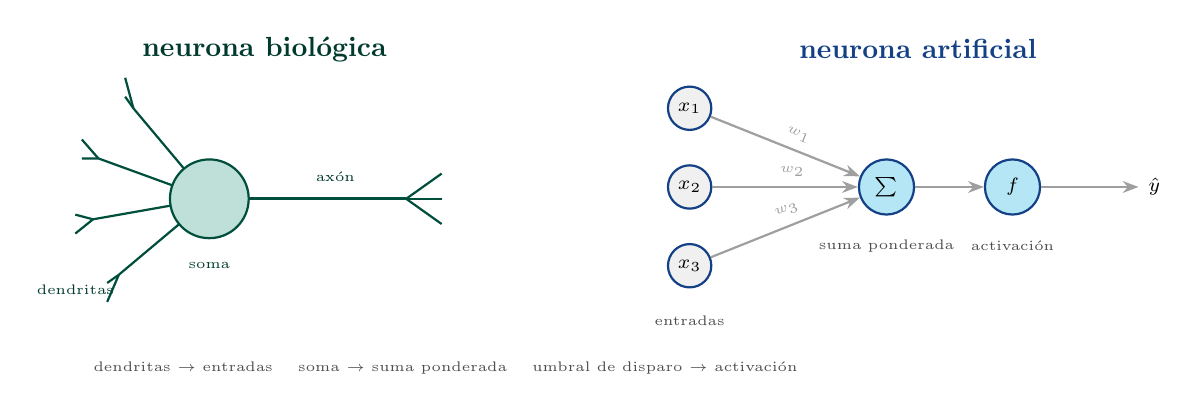
\begin{tikzpicture}[font=\scriptsize,
	fl/.style={-{Stealth[length=2mm]}, thick, gray!75},
	ent/.style={circle, draw=UCMNavy, thick, fill=LightGray, minimum size=5.5mm, inner sep=0pt},
	op/.style={circle, draw=UCMNavy, thick, fill=UCMBlue!30, minimum size=7mm, inner sep=0pt}]

	% ---------- neurona biológica ----------
	\begin{scope}[xshift=0cm]
		\fill[AccentGreen!25, draw=AccentGreen!60!black, thick] (0,0) circle (0.5);
		\foreach \a in {130,160,190,220}{
			\draw[AccentGreen!60!black, thick] (\a:0.5) -- (\a:1.5);
			\draw[AccentGreen!60!black, thick] (\a:1.5) -- ++($(\a:0.35)+(0.12,0.12)$);
			\draw[AccentGreen!60!black, thick] (\a:1.5) -- ++($(\a:0.35)+(0.12,-0.12)$);
		}
		\draw[AccentGreen!60!black, very thick] (0.5,0) -- (2.5,0);
		\foreach \dy in {0.32,0,-0.32}{\draw[AccentGreen!60!black, thick] (2.5,0) -- (2.95,\dy);}
		\node[font=\tiny, text=AccentGreen!45!black] at (-1.7,-1.15) {dendritas};
		\node[font=\tiny, text=AccentGreen!45!black] at (0,-0.85) {soma};
		\node[font=\tiny, text=AccentGreen!45!black] at (1.6,0.28) {ax\'on};
		\node[font=\bfseries, text=AccentGreen!45!black] at (0.7,1.9) {neurona biol\'ogica};
	\end{scope}

	% ---------- neurona artificial ----------
	\begin{scope}[xshift=6.1cm]
		\node[ent] (x1) at (0,1.15)  {$x_1$};
		\node[ent] (x2) at (0,0.15)  {$x_2$};
		\node[ent] (x3) at (0,-0.85) {$x_3$};
		\node[op]  (su) at (2.5,0.15) {$\sum$};
		\node[op]  (fa) at (4.1,0.15) {$f$};
		\node (out) at (5.9,0.15) {$\hat y$};
		\foreach \i/\w in {1/{$w_1$},2/{$w_2$},3/{$w_3$}}{
			\draw[fl] (x\i) -- node[above, font=\tiny, pos=0.55, sloped] {\w} (su);
		}
		\draw[fl] (su) -- (fa);
		\draw[fl] (fa) -- (out);
		\node[font=\tiny, text=StanfordGray] at (0,-1.55) {entradas};
		\node[font=\tiny, text=StanfordGray] at (2.5,-0.6) {suma ponderada};
		\node[font=\tiny, text=StanfordGray] at (4.1,-0.6) {activaci\'on};
		\node[font=\bfseries, text=UCMNavy] at (2.9,1.9) {neurona artificial};
	\end{scope}

	% ---------- correspondencias ----------
	\node[font=\tiny, text=StanfordGray] at (3.0,-2.15)
		{dendritas $\to$ entradas \quad soma $\to$ suma ponderada \quad umbral de disparo $\to$ activaci\'on};
\end{tikzpicture}}
\end{center}
\vspace{0.1em}
\idea{La analog\'ia motiva el modelo, pero no lo justifica. El cerebro tiene $\sim\!10^{11}$ neuronas con din\'amica temporal, neurotransmisores y plasticidad local: nada de eso est\'a en $f(\mathbf{w}^{\mathrm{T}}\mathbf{x})$. Es un \textbf{modelo inspirado} en la biolog\'ia, no una simulaci\'on de ella.}
\end{frame}

\begin{frame}
\frametitle{¿Qué significa aprender?}
\begin{block}{Agente que aprende}
Un agente \textbf{aprende} si, dado un modelo y un criterio de optimizaci\'on, mejora su desempe\~no al recibir nueva informaci\'on.
\end{block}
\pause
\begin{columns}[T]
\begin{column}{6cm}
\begin{itemize}
	\item Del conjunto de \textbf{entrenamiento} el agente construye un mapa entre las caracter\'isticas observadas y la respuesta.
	\item Ante datos nuevos, cuya respuesta desconoce, usa ese mapa para \textbf{generalizar}.
\end{itemize}
\end{column}
\begin{column}{6cm}
\formula{\centering
$\displaystyle \min_{\mathbf w} \; \frac{1}{n}\sum_{i=1}^{n} \ell\big(f_{\mathbf w}(\mathbf x_i),\, y_i\big)$}
\footnotesize
Todo lo que sigue en esta clase es \emph{una} elecci\'on concreta de $f_{\mathbf w}$ y de $\ell$.
\end{column}
\end{columns}
\vspace{0.3em}
\idea{Ajustar bien el conjunto de entrenamiento es f\'acil y no es el objetivo. El objetivo es el error en datos \textbf{no vistos}.}
\end{frame}

\begin{frame}
\frametitle{Aprendizaje supervisado: dos tareas}
Dado $\mathcal D = \{(\mathbf x_i, y_i)\}_{i=1}^{n}$, la diferencia est\'a en la \textbf{naturaleza de $y$}:
\vspace{0.2em}
\begin{columns}[T]
\begin{column}{6.1cm}
\begin{center}
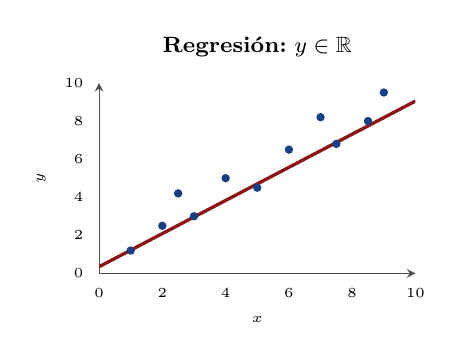
\begin{tikzpicture}
\begin{axis}[width=5.6cm, height=4.0cm, title={\footnotesize\textbf{Regresi\'on:} $y \in \mathbb{R}$},
	xlabel={$x$}, ylabel={$y$}, xlabel style={font=\tiny}, ylabel style={font=\tiny},
	tick label style={font=\tiny}, axis lines=left, xmin=0, xmax=10, ymin=0, ymax=10,
	axis line style={StanfordGray}, tick style={draw=none}]
	\addplot[only marks, mark=*, mark size=1.3pt, UCMNavy] coordinates {
		(1,1.2) (2,2.5) (2.5,4.2) (3,3.0) (4,5.0) (5,4.5) (6,6.5) (7,8.2) (7.5,6.8) (8.5,8.0) (9,9.5)};
	\addplot[StanfordRed, very thick, domain=0:10]{0.87*x+0.35};
\end{axis}
\end{tikzpicture}
\end{center}
\footnotesize\centering predecir un \textbf{valor}
\end{column}
\begin{column}{6.1cm}
\begin{center}
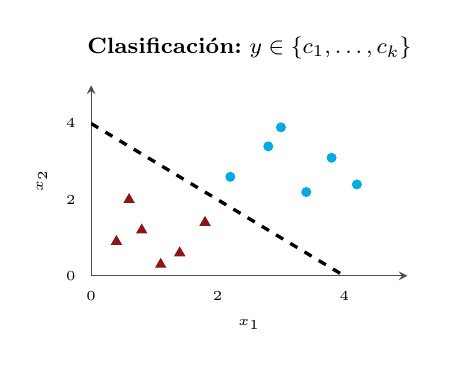
\begin{tikzpicture}
\begin{axis}[width=5.6cm, height=4.0cm, title={\footnotesize\textbf{Clasificaci\'on:} $y \in \{c_1,\ldots,c_k\}$},
	xlabel={$x_1$}, ylabel={$x_2$}, xlabel style={font=\tiny}, ylabel style={font=\tiny},
	tick label style={font=\tiny}, axis lines=left, xmin=0, xmax=5, ymin=0, ymax=5,
	axis line style={StanfordGray}, tick style={draw=none}]
	\addplot[only marks, mark=*, mark size=1.6pt, UCMBlue] coordinates {
		(2.2,2.6) (2.8,3.4) (3.4,2.2) (3.0,3.9) (3.8,3.1) (4.2,2.4)};
	\addplot[only marks, mark=triangle*, mark size=2pt, StanfordRed] coordinates {
		(0.8,1.2) (1.4,0.6) (0.6,2.0) (1.8,1.4) (1.1,0.3) (0.4,0.9)};
	\addplot[black, very thick, dashed, domain=0:5]{4-x};
\end{axis}
\end{tikzpicture}
\end{center}
\footnotesize\centering asignar una \textbf{categor\'ia}
\end{column}
\end{columns}
\vspace{0.2em}
\idea{Misma maquinaria, distinto $\ell$: el error cuadr\'atico para valores continuos, la entrop\'ia cruzada para categor\'ias. Lo veremos al final de la clase.}
\end{frame}

%=====================================================================
\section{Regresión: capacidad y generalización}
%=====================================================================

\begin{frame}
\frametitle{Regresión polinomial}
\begin{itemize}
	\item Para regresi\'on no lineal en una variable, ajustamos un polinomio de orden $p$:
\end{itemize}
\formula{
\[
y = f(x) + \epsilon = w_0 + \sum_{j=1}^{p} w_j x^{j} + \epsilon,
\qquad \epsilon \sim \mathcal{N}(0,\sigma^2)
\]}
\pause
\begin{itemize}
	\item Los par\'ametros $\mathbf w = [w_0,\ldots,w_p]$ se obtienen por \textbf{m\'inimos cuadrados}:
\end{itemize}
\formula{
\[
E_p(\mathbf w) = \frac{1}{n}\sum_{i=1}^{n}\big(y_i - f(x_i)\big)^{2}
\]}
\pause
\begin{itemize}
	\item El modelo es \textbf{no lineal en $x$} pero \textbf{lineal en $\mathbf w$}: por eso tiene soluci\'on cerrada, $\mathbf w^\star = (\mathbf X^{\mathrm{T}}\mathbf X)^{-1}\mathbf X^{\mathrm{T}}\mathbf y$.
	\item $p$ no se aprende de los datos: es un \textbf{hiperpar\'ametro} que fija la \emph{capacidad} del modelo.
\end{itemize}
\end{frame}

\begin{frame}
\frametitle{Los mismos datos, tres capacidades}
\begin{center}
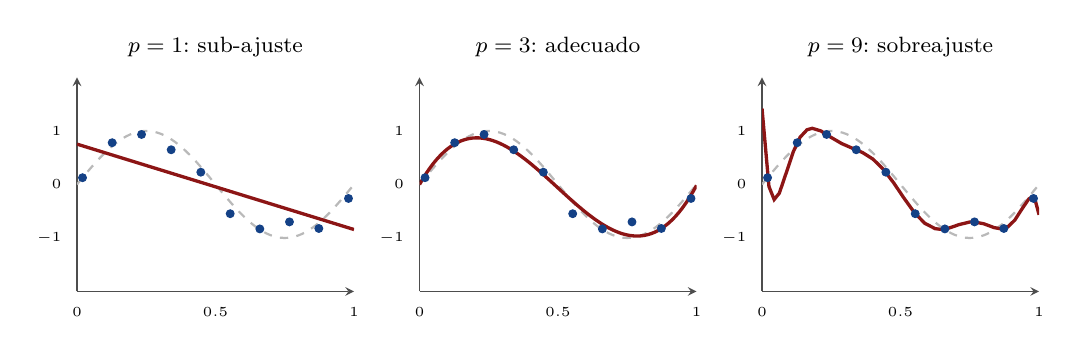
\begin{tikzpicture}[font=\scriptsize]
\foreach \p/\tit/\xs in {0/{$p=1$: sub-ajuste}/0, 1/{$p=3$: adecuado}/4.35, 2/{$p=9$: sobreajuste}/8.7}{
\begin{scope}[xshift=\xs cm]
\begin{axis}[width=5.1cm, height=4.3cm, title={\footnotesize \tit},
	xmin=0, xmax=1, ymin=-2, ymax=2, axis lines=left,
	xtick={0,0.5,1}, ytick={-1,0,1}, tick label style={font=\tiny},
	axis line style={StanfordGray}, tick style={draw=none},
	title style={font=\scriptsize, yshift=-2pt}]
	\addplot[gray!55, dashed, thick, domain=0:1, samples=80]{sin(deg(2*pi*x))};
	\addplot[only marks, mark=*, mark size=1.4pt, UCMNavy] coordinates {
		(0.020,0.126) (0.127,0.780) (0.233,0.934) (0.340,0.648) (0.447,0.229)
		(0.553,-0.547) (0.660,-0.831) (0.767,-0.700) (0.873,-0.823) (0.980,-0.262)};
	\ifnum\p=0
		\addplot[StanfordRed, very thick, domain=0:1, samples=2]{-1.5961*x+0.7535};
	\fi
	\ifnum\p=1
		\addplot[StanfordRed, very thick, domain=0:1, samples=80]
			{18.9715*x^3-28.2296*x^2+9.2426*x-0.0012};
	\fi
	\ifnum\p=2
		\addplot[StanfordRed, very thick] coordinates {
			(0.0000,1.418) (0.0250,-0.038) (0.0438,-0.282) (0.0625,-0.162) (0.0875,0.219)
			(0.1125,0.607) (0.1375,0.883) (0.1625,1.022) (0.1813,1.049) (0.2125,1.000)
			(0.2500,0.877) (0.2875,0.764) (0.3250,0.679) (0.3625,0.597) (0.4000,0.475)
			(0.4375,0.286) (0.4750,0.031) (0.5125,-0.256) (0.5500,-0.526) (0.5875,-0.726)
			(0.6250,-0.826) (0.6438,-0.838) (0.6750,-0.814) (0.7125,-0.749) (0.7500,-0.702)
			(0.7625,-0.699) (0.8000,-0.734) (0.8375,-0.806) (0.8625,-0.830) (0.8875,-0.792)
			(0.9125,-0.666) (0.9375,-0.464) (0.9625,-0.274) (0.9688,-0.251) (0.9750,-0.247)
			(0.9875,-0.323) (1.0000,-0.567)};
	\fi
\end{axis}
\end{scope}}
\end{tikzpicture}
\end{center}
\vspace{-0.2em}
\footnotesize\centering
{\color{StanfordGray} l\'inea gris: la funci\'on real $\sin(2\pi x)$ \quad$\bullet$\quad puntos: 10 observaciones con ruido \quad$\bullet$\quad rojo: el polinomio ajustado}
\vspace{0.2em}
\idea{Con $p=9$ y 10 puntos el ajuste es \textbf{perfecto} sobre los datos de entrenamiento (error cero) y sin embargo el modelo es peor. El error de entrenamiento no mide lo que nos importa.}
\end{frame}

\begin{frame}
\frametitle{La curva en U: capacidad vs. generalización}
\begin{columns}[c]
\begin{column}{6.6cm}
\begin{center}
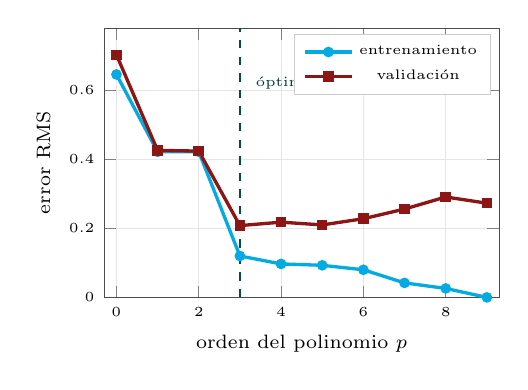
\begin{tikzpicture}
\begin{axis}[width=6.6cm, height=5.0cm,
	xlabel={orden del polinomio $p$}, ylabel={error RMS},
	xlabel style={font=\scriptsize}, ylabel style={font=\scriptsize},
	tick label style={font=\tiny}, xmin=-0.3, xmax=9.3, ymin=0, ymax=0.78,
	legend style={font=\tiny, at={(0.98,0.98)}, anchor=north east, draw=gray!40},
	grid=major, grid style={gray!20}, axis line style={StanfordGray}]
	\addplot[UCMBlue, very thick, mark=*, mark size=1.3pt] coordinates {
		(0,0.646) (1,0.422) (2,0.422) (3,0.120) (4,0.097) (5,0.093)
		(6,0.080) (7,0.042) (8,0.026) (9,0.000)};
	\addplot[StanfordRed, very thick, mark=square*, mark size=1.3pt] coordinates {
		(0,0.703) (1,0.426) (2,0.424) (3,0.208) (4,0.218) (5,0.210)
		(6,0.228) (7,0.256) (8,0.291) (9,0.273)};
	\legend{entrenamiento, validaci\'on}
	\draw[AccentGreen!60!black, thick, dashed] (axis cs:3,0) -- (axis cs:3,0.78);
	\node[AccentGreen!45!black, font=\tiny, anchor=west] at (axis cs:3.15,0.62) {\'optimo};
\end{axis}
\end{tikzpicture}
\end{center}
\end{column}
\begin{column}{5.6cm}
\begin{itemize}
	\item El error de \textbf{entrenamiento} baja de forma mon\'otona: m\'as capacidad siempre ajusta mejor lo ya visto.
	\item El error de \textbf{validaci\'on} baja, toca un m\'inimo y vuelve a subir: ah\'i empieza el sobreajuste.
	\item La distancia entre ambas curvas es la \textbf{brecha de generalizaci\'on}.
\end{itemize}
\vspace{0.3em}
\footnotesize
Herramientas para controlarla: m\'as datos, regularizaci\'on, detenci\'on temprana. Es el tema de la clase 1.4.
\end{column}
\end{columns}
\vspace{0.2em}
\idea{La capacidad \'optima no es la m\'axima ni la m\'inima: se \textbf{elige}, y se elige midiendo sobre datos que el modelo no us\'o para ajustarse.}
\end{frame}

%=====================================================================
\section{Clasificación: el perceptrón}
%=====================================================================

\begin{frame}
\frametitle{El perceptrón}
\begin{columns}[T]
\begin{column}{6.2cm}
\begin{itemize}
	\item Clasificaci\'on binaria con entradas $\mathbf x \in \mathbb{R}^{D}$ y etiqueta $y \in \{-1,+1\}$.
	\item Los $w_j$ son los \textbf{pesos} y $w_0$ el \textbf{sesgo}.
\end{itemize}
\formula{
\[
f(\mathbf x) = f\Big(w_0 + \sum_{j=1}^{D} w_j x_j\Big) = f(\mathbf w^{\mathrm{T}}\mathbf x)
\]}
\pause
\begin{itemize}
	\item Rosenblatt (1958) usa como activaci\'on la \textbf{funci\'on signo}:
\end{itemize}
\formula{
\[
f(\mathbf x) =
\begin{cases}
+1 & \mathbf w^{\mathrm{T}}\mathbf x \geq 0\\
-1 & \mathbf w^{\mathrm{T}}\mathbf x < 0
\end{cases}
\]}
\end{column}
\begin{column}{6.0cm}
\begin{center}
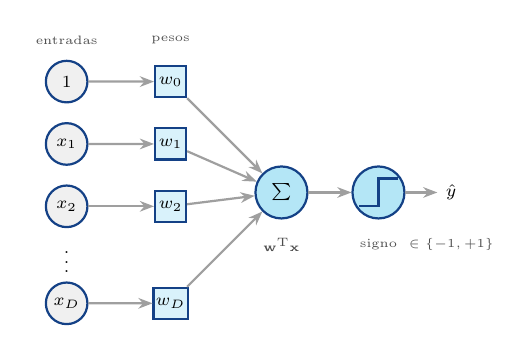
\begin{tikzpicture}[font=\scriptsize, scale=0.88, transform shape,
	ent/.style={circle, draw=UCMNavy, thick, fill=LightGray, minimum size=6mm, inner sep=0pt},
	peso/.style={rectangle, draw=UCMNavy, thick, fill=UCMBlue!15, minimum size=4.5mm, inner sep=1pt},
	op/.style={circle, draw=UCMNavy, thick, fill=UCMBlue!30, minimum size=7.5mm, inner sep=0pt},
	fl/.style={-{Stealth[length=1.8mm]}, thick, gray!75}]

	\node[ent] (x0) at (0, 1.95) {$1$};
	\node[ent] (x1) at (0, 1.05) {$x_1$};
	\node[ent] (x2) at (0, 0.15) {$x_2$};
	\node       (pt) at (0,-0.55) {$\vdots$};
	\node[ent] (xd) at (0,-1.25) {$x_D$};

	\node[peso] (w0) at (1.5, 1.95) {$w_0$};
	\node[peso] (w1) at (1.5, 1.05) {$w_1$};
	\node[peso] (w2) at (1.5, 0.15) {$w_2$};
	\node[peso] (wd) at (1.5,-1.25) {$w_D$};

	\node[op] (su) at (3.1, 0.35) {$\sum$};
	\node[op] (fa) at (4.5, 0.35) {};
	% función escalón dentro del nodo de activación
	\draw[UCMNavy, thick] ($(fa)+(-0.28,-0.2)$) -- ($(fa)+(0,-0.2)$) -- ($(fa)+(0,0.2)$) -- ($(fa)+(0.28,0.2)$);
	\node (out) at (5.55, 0.35) {$\hat y$};
	\node[font=\tiny, text=StanfordGray] at (5.55,-0.4) {$\in\{-1,+1\}$};

	\foreach \i in {0,1,2,d}{\draw[fl] (x\i) -- (w\i); \draw[fl] (w\i) -- (su);}
	\draw[fl] (su) -- (fa);
	\draw[fl] (fa) -- (out);

	\node[font=\tiny, text=StanfordGray] at (0, 2.55) {entradas};
	\node[font=\tiny, text=StanfordGray] at (1.5, 2.55) {pesos};
	\node[font=\tiny, text=StanfordGray] at (3.1,-0.4) {$\mathbf w^{\mathrm{T}}\mathbf x$};
	\node[font=\tiny, text=StanfordGray] at (4.5,-0.4) {signo};
\end{tikzpicture}
\end{center}
\end{column}
\end{columns}
\end{frame}

\begin{frame}
\frametitle{Qué significa geométricamente}
\begin{columns}[c]
\begin{column}{6.1cm}
\begin{center}
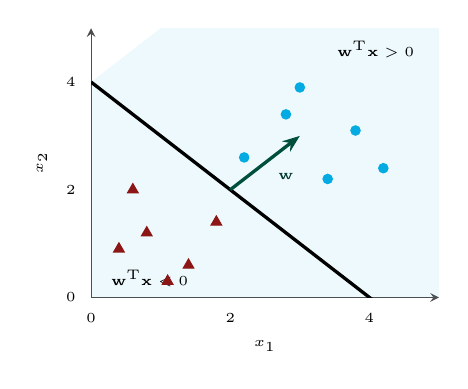
\begin{tikzpicture}
\begin{axis}[width=6.0cm, height=5.0cm, xlabel={$x_1$}, ylabel={$x_2$},
	xlabel style={font=\tiny}, ylabel style={font=\tiny},
	tick label style={font=\tiny}, axis lines=left, xmin=0, xmax=5, ymin=0, ymax=5,
	axis line style={StanfordGray}, tick style={draw=none}]
	\addplot[fill=UCMBlue, opacity=0.07, draw=none] coordinates {(0,4)(1,5)(5,5)(5,0)(4,0)} \closedcycle;
	\addplot[only marks, mark=*, mark size=1.7pt, UCMBlue] coordinates {
		(2.2,2.6) (2.8,3.4) (3.4,2.2) (3.0,3.9) (3.8,3.1) (4.2,2.4)};
	\addplot[only marks, mark=triangle*, mark size=2.2pt, StanfordRed] coordinates {
		(0.8,1.2) (1.4,0.6) (0.6,2.0) (1.8,1.4) (1.1,0.3) (0.4,0.9)};
	\addplot[black, very thick, domain=0:5, samples=2]{4-x};
	\draw[-{Stealth[length=2.2mm]}, very thick, AccentGreen!60!black]
		(axis cs:2,2) -- (axis cs:3.0,3.0);
	\node[font=\tiny, text=AccentGreen!45!black, anchor=west] at (axis cs:2.55,2.25) {$\mathbf w$};
	\node[font=\tiny, anchor=west] at (axis cs:3.4,4.6) {$\mathbf w^{\mathrm{T}}\mathbf x > 0$};
	\node[font=\tiny, anchor=west] at (axis cs:0.15,0.35) {$\mathbf w^{\mathrm{T}}\mathbf x < 0$};
\end{axis}
\end{tikzpicture}
\end{center}
\end{column}
\begin{column}{5.9cm}
\begin{itemize}
	\item La ecuaci\'on $\mathbf w^{\mathrm{T}}\mathbf x = 0$ define un \textbf{hiperplano}: una recta en $\mathbb{R}^2$, un plano en $\mathbb{R}^3$.
	\item El vector $\mathbf w$ es \textbf{perpendicular} a ese hiperplano y apunta hacia la clase $+1$.
	\item El sesgo $w_0$ desplaza el hiperplano sin cambiar su orientaci\'on.
	\item Clasificar es preguntar \textbf{de qu\'e lado} cae el punto.
\end{itemize}
\end{column}
\end{columns}
\vspace{0.2em}
\idea{El perceptr\'on solo puede trazar \textbf{una} frontera recta. Toda la clase se juega en esa limitaci\'on.}
\end{frame}

\begin{frame}
\frametitle{La regla de aprendizaje}
\begin{itemize}
	\item Los patrones bien clasificados aportan error cero. Para los mal clasificados ($i \in \mathcal M$) se cumple $\mathbf w^{\mathrm{T}}\mathbf x_i y_i < 0$, as\'i que minimizamos
\end{itemize}
\formula{
\[
E(\mathbf w) = -\sum_{i \in \mathcal M} \mathbf w^{\mathrm{T}}\mathbf x_i\, y_i \;\geq\; 0
\]}
\pause
\begin{itemize}
	\item El entrenamiento usa \textbf{descenso de gradiente}:
\end{itemize}
\formula{
\[
\mathbf w^{\tau+1} = \mathbf w^{\tau} - \eta\,\nabla E(\mathbf w^{\tau})
= \mathbf w^{\tau} + \eta \sum_{i \in \mathcal M} \mathbf x_i\, y_i
\]}
\pause
\begin{itemize}
	\item $\eta > 0$ es la \textbf{tasa de aprendizaje} y $\tau$ el n\'umero de iteraci\'on.
	\item Solo los ejemplos \textbf{mal clasificados} modifican los pesos: un patr\'on correcto no aporta nada al gradiente.
\end{itemize}
\end{frame}

\begin{frame}
\frametitle{Por qué funciona la regla}
\begin{columns}[c]
\begin{column}{6.0cm}
\begin{center}
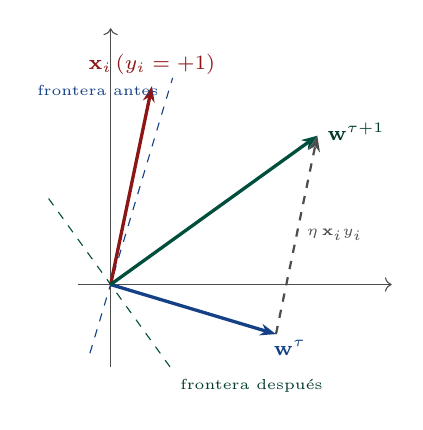
\begin{tikzpicture}[font=\scriptsize, scale=1.05, transform shape]
	\draw[StanfordGray, ->] (-0.4,0) -- (3.4,0);
	\draw[StanfordGray, ->] (0,-1.0) -- (0,3.1);

	% w antes y su frontera
	\draw[-{Stealth[length=2mm]}, very thick, UCMNavy] (0,0) -- (2.0,-0.6);
	\node[UCMNavy, font=\scriptsize, anchor=north west] at (1.85,-0.55) {$\mathbf w^{\tau}$};
	\draw[UCMNavy, dashed] (-0.25,-0.83) -- (0.75,2.5);

	% el patrón mal clasificado (y=+1)
	\draw[-{Stealth[length=2mm]}, very thick, StanfordRed] (0,0) -- (0.5,2.4);
	\node[StanfordRed, font=\scriptsize, anchor=south] at (0.5,2.42) {$\mathbf x_i\,(y_i=+1)$};

	% actualización
	\draw[-{Stealth[length=2mm]}, thick, StanfordGray, dashed] (2.0,-0.6) -- (2.5,1.8);
	\node[StanfordGray, font=\tiny, anchor=west] at (2.25,0.6) {$\eta\,\mathbf x_i y_i$};
	\draw[-{Stealth[length=2mm]}, very thick, AccentGreen!60!black] (0,0) -- (2.5,1.8);
	\node[AccentGreen!45!black, font=\scriptsize, anchor=west] at (2.5,1.85) {$\mathbf w^{\tau+1}$};
	% frontera nueva: perpendicular a w^{tau+1}
	\draw[AccentGreen!60!black, dashed] (-0.75,1.04) -- (0.75,-1.04);
	\node[UCMNavy, font=\tiny, anchor=east] at (0.7,2.35) {frontera antes};
	\node[AccentGreen!45!black, font=\tiny, anchor=north west] at (0.72,-1.02) {frontera despu\'es};
\end{tikzpicture}
\end{center}
\end{column}
\begin{column}{6.2cm}
\begin{itemize}
	\item $\mathbf x_i$ pertenece a la clase $+1$ pero cae del lado negativo de $\mathbf w^{\tau}$: est\'a \textbf{mal clasificado}.
	\item La actualizaci\'on suma $\eta\,\mathbf x_i y_i$, es decir \textbf{rota $\mathbf w$ hacia el patr\'on}.
	\item Tras el paso, $\mathbf w^{\tau+1\,\mathrm{T}}\mathbf x_i = \mathbf w^{\tau\,\mathrm{T}}\mathbf x_i + \eta\lVert\mathbf x_i\rVert^{2}$: el producto \emph{siempre} aumenta.
	\item Si la etiqueta fuera $-1$, la regla restar\'ia $\mathbf x_i$ y alejar\'ia el vector.
\end{itemize}
\end{column}
\end{columns}
\vspace{0.2em}
\idea{Cada correcci\'on mejora el margen \emph{de ese} patr\'on, aunque pueda estropear otros. La garant\'ia global la da el teorema de convergencia.}
\end{frame}

\begin{frame}
\frametitle{Convergencia y sus límites}
\begin{columns}[T]
\begin{column}{6.1cm}
\begin{exampleblock}{Teorema de convergencia}
Si las clases son \textbf{linealmente separables}, la regla del perceptr\'on encuentra una soluci\'on en un n\'umero \textbf{finito} de pasos, cualquiera sea la inicializaci\'on.
\end{exampleblock}
\end{column}
\begin{column}{6.1cm}
\begin{alertblock}{La letra chica}
\begin{itemize}
	\item Si \emph{no} son separables, el algoritmo \textbf{no converge}: oscila indefinidamente.
	\item La soluci\'on encontrada no es \'unica ni la de mayor margen: depende del orden de los datos.
	\item No se extiende de forma natural a m\'as de dos clases.
	\item La salida es una decisi\'on dura: no dice \emph{cu\'an seguro} est\'a.
\end{itemize}
\end{alertblock}
\end{column}
\end{columns}
\vspace{0.4em}
\footnotesize
Los dos \'ultimos problemas se resuelven cambiando la funci\'on de activaci\'on. El primero, cambiando la arquitectura.
\end{frame}

%=====================================================================
\section{De la decisión dura a la probabilidad}
%=====================================================================

\begin{frame}
\frametitle{Clasificación probabilística}
\begin{itemize}
	\item El signo devuelve un lado, no una confianza. Modelemos ahora $p(y=1\mid\mathbf x)$.
	\item Cambiamos de codificaci\'on: de aqu\'i en adelante $y\in\{0,1\}$ en lugar de $\{-1,+1\}$.
	\item Postulamos que el \textbf{logaritmo de la raz\'on de momios} es lineal en $\mathbf x$:
\end{itemize}
\formula{
\[
\log\!\left(\frac{p(y=1\mid\mathbf x)}{p(y=0\mid\mathbf x)}\right) = \mathbf w^{\mathrm{T}}\mathbf x
\]}
\pause
\begin{itemize}
	\item Despejando se obtiene la \textbf{funci\'on log\'istica} (sigmoide):
\end{itemize}
\formula{
\[
\begin{aligned}
p(y=1\mid\mathbf x) &= \sigma(\mathbf w^{\mathrm{T}}\mathbf x)
= \frac{\exp(\mathbf w^{\mathrm{T}}\mathbf x)}{1+\exp(\mathbf w^{\mathrm{T}}\mathbf x)}
= \frac{1}{1+\exp(-\mathbf w^{\mathrm{T}}\mathbf x)}\\[2pt]
p(y=0\mid\mathbf x) &= 1-\sigma(\mathbf w^{\mathrm{T}}\mathbf x)
\end{aligned}
\]}
\vspace{0.1em}
\footnotesize
Las dos expresiones de $\sigma$ son equivalentes: basta dividir numerador y denominador por $\exp(\mathbf w^{\mathrm{T}}\mathbf x)$. Ojo con el \textbf{signo del exponente}.
\end{frame}

\begin{frame}
\frametitle{La función sigmoide}
\begin{columns}[T]
\begin{column}{6.0cm}
\begin{itemize}
	\item $\sigma:\mathbb{R}\mapsto(0,1)$, as\'i que la salida se lee como probabilidad.
	\item Es continua y diferenciable: habilita el descenso de gradiente, que el escal\'on del perceptr\'on imped\'ia.
	\item Su derivada se escribe en t\'erminos de s\'i misma:
\end{itemize}
\formula{\footnotesize
\[
\begin{aligned}
\sigma'(z) &= \sigma(z)\big(1-\sigma(z)\big)\\[2pt]
\frac{\partial}{\partial \mathbf w}\,\sigma(\mathbf w^{\mathrm{T}}\mathbf x)
&= \sigma(1-\sigma)\,\mathbf x
\end{aligned}
\]}
\footnotesize
El factor $\mathbf x$ viene de la regla de la cadena: no lo olvide al derivar respecto de los \emph{pesos}.
\end{column}
\begin{column}{6.1cm}
\begin{center}
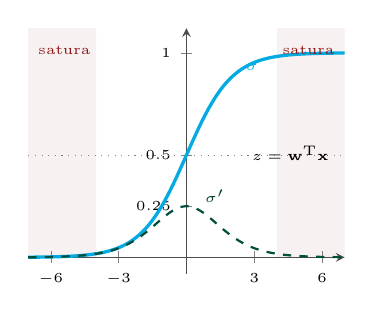
\begin{tikzpicture}
\begin{axis}[width=5.6cm, height=4.7cm, axis lines=middle,
	xlabel={$z=\mathbf w^{\mathrm{T}}\mathbf x$}, xlabel style={font=\tiny, at={(axis description cs:0.98,0.42)}},
	xmin=-7, xmax=7, ymin=-0.08, ymax=1.12,
	ytick={0,0.25,0.5,1}, xtick={-6,-3,0,3,6},
	tick label style={font=\tiny}, axis line style={StanfordGray}]
	\addplot[fill=StanfordRed, opacity=0.06, draw=none] coordinates {(-7,0)(-4,0)(-4,1.12)(-7,1.12)} \closedcycle;
	\addplot[fill=StanfordRed, opacity=0.06, draw=none] coordinates {(4,0)(7,0)(7,1.12)(4,1.12)} \closedcycle;
	\addplot[UCMBlue, very thick, domain=-7:7, samples=200]{1/(1+exp(-x))};
	\addplot[AccentGreen!60!black, thick, dashed, domain=-7:7, samples=200]
		{(1/(1+exp(-x)))*(1-(1/(1+exp(-x))))};
	\draw[gray, dotted] (axis cs:-7,0.5) -- (axis cs:7,0.5);
	\node[font=\tiny, text=StanfordRed, anchor=north] at (axis cs:-5.4,1.08) {satura};
	\node[font=\tiny, text=StanfordRed, anchor=north] at (axis cs:5.4,1.08) {satura};
	\node[font=\tiny, text=AccentGreen!45!black, anchor=west] at (axis cs:0.4,0.30) {$\sigma'$};
	\node[font=\tiny, text=UCMBlue, anchor=west] at (axis cs:2.2,0.93) {$\sigma$};
\end{axis}
\end{tikzpicture}
\end{center}
\end{column}
\end{columns}
\vspace{0.1em}
\idea{En las colas $\sigma'\!\to\!0$: el gradiente se desvanece y el aprendizaje se detiene. Este defecto reaparecer\'a al apilar capas y motivar\'a ReLU.}
\end{frame}

\begin{frame}
\frametitle{La pérdida: entropía cruzada}
La verosimilitud de una etiqueta Bernoulli es $p^{y}(1-p)^{1-y}$. Tomando $-\log$ y promediando:
\formula{
\[
E(\mathbf w) = \frac{1}{n}\sum_{i=1}^{n}
\Big[-y_i \log \sigma(\mathbf w^{\mathrm{T}}\mathbf x_i) - (1-y_i)\log\big(1-\sigma(\mathbf w^{\mathrm{T}}\mathbf x_i)\big)\Big]
\]}
\pause
\begin{columns}[T]
\begin{column}{6.1cm}
\begin{block}{Regresión (error cuadrático)}
\[
\nabla E = \frac{2}{n}\sum_i \big(\hat y_i - y_i\big)\,\mathbf x_i
\]
\end{block}
\end{column}
\begin{column}{6.1cm}
\begin{block}{Clasificación (entropía cruzada)}
\[
\nabla E = \frac{1}{n}\sum_i \big(\sigma(\mathbf w^{\mathrm{T}}\mathbf x_i) - y_i\big)\,\mathbf x_i
\]
\end{block}
\end{column}
\end{columns}
\vspace{0.4em}
\idea{Distinto modelo y distinta p\'erdida, \textbf{misma forma del gradiente}: (predicci\'on $-$ objetivo) $\times$ entrada. No es casualidad, y es lo que hace que un mismo optimizador sirva para todo el curso.}
\end{frame}

%=====================================================================
\section{El límite del perceptrón}
%=====================================================================

\begin{frame}
\frametitle{El problema XOR}
\begin{columns}[c]
\begin{column}{6.4cm}
\begin{center}
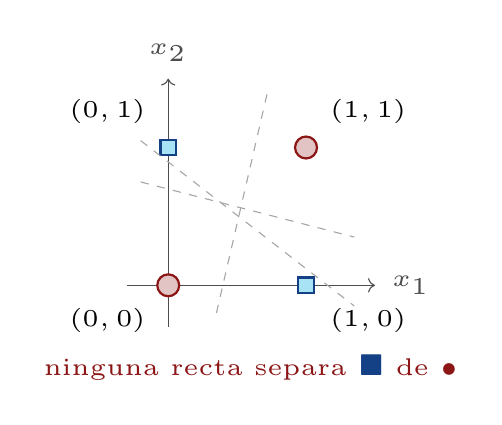
\begin{tikzpicture}[font=\scriptsize, scale=1.75, transform shape]
	\draw[StanfordGray, ->] (-0.3,0) -- (1.5,0) node[right, font=\tiny] {$x_1$};
	\draw[StanfordGray, ->] (0,-0.3) -- (0,1.5) node[above, font=\tiny] {$x_2$};
	\foreach \x/\y in {0/0, 1/1}
		\node[circle, draw=StanfordRed, thick, fill=StanfordRed!25, inner sep=1.6pt] at (\x,\y) {};
	\foreach \x/\y in {0/1, 1/0}
		\node[rectangle, draw=UCMNavy, thick, fill=UCMBlue!35, inner sep=1.6pt] at (\x,\y) {};
	\node[font=\tiny, anchor=north east] at (-0.04,-0.04) {$(0,0)$};
	\node[font=\tiny, anchor=south west] at (1.05,1.05) {$(1,1)$};
	\node[font=\tiny, anchor=south east] at (-0.04,1.05) {$(0,1)$};
	\node[font=\tiny, anchor=north west] at (1.05,-0.04) {$(1,0)$};
	% tres rectas que fracasan
	\draw[gray!70, dashed] (-0.2,0.75) -- (1.35,0.35);
	\draw[gray!70, dashed] (0.35,-0.2) -- (0.72,1.4);
	\draw[gray!70, dashed] (-0.2,1.05) -- (1.35,-0.15);
	\node[font=\tiny, text=StanfordRed] at (0.6,-0.6)
		{ninguna recta separa \textcolor{UCMNavy}{$\blacksquare$} de \textcolor{StanfordRed}{$\bullet$}};
\end{tikzpicture}
\end{center}
\end{column}
\begin{column}{5.8cm}
\footnotesize
\begin{center}
\begin{tabular}{ccc}
\toprule
$x_1$ & $x_2$ & $y = x_1 \oplus x_2$\\
\midrule
0 & 0 & 0\\
0 & 1 & 1\\
1 & 0 & 1\\
1 & 1 & 0\\
\bottomrule
\end{tabular}
\end{center}
\vspace{0.4em}
\begin{itemize}
	\item AND y OR \emph{s\'i} son linealmente separables; XOR no.
	\item Un perceptr\'on no puede aprender la funci\'on l\'ogica m\'as simple que no es lineal.
\end{itemize}
\end{column}
\end{columns}
\vspace{0.2em}
\idea{Bastan \textbf{dos} rectas para resolverlo: una capa oculta de dos neuronas m\'as una de salida. Ese es exactamente el perceptr\'on multicapa de la pr\'oxima clase.}
\end{frame}

\begin{frame}
\frametitle{Minsky, Papert y el primer invierno}
\begin{columns}[T]
\begin{column}{6.1cm}
\begin{itemize}
	\item En \emph{Perceptrons} (1969), Minsky y Papert demostraron formalmente esta limitaci\'on.
	\item El libro tambi\'en se\~nal\'o que no exist\'ia entonces un algoritmo de entrenamiento para redes \textbf{multicapa}.
	\item El financiamiento a redes neuronales se desplom\'o: es el \textbf{primer invierno de la IA} que vimos en la clase 1.1.
\end{itemize}
\end{column}
\begin{column}{6.1cm}
\begin{exampleblock}{Lo que faltaba}
La respuesta lleg\'o en 1986 con la popularizaci\'on de la \textbf{retropropagaci\'on} (Rumelhart, Hinton y Williams): una forma eficiente de calcular el gradiente en redes de varias capas.
\end{exampleblock}
\vspace{0.2em}
\footnotesize
Entre el diagn\'ostico del problema y su soluci\'on pasaron \textbf{diecisiete a\~nos}.
\end{column}
\end{columns}
\vspace{0.4em}
\idea{La limitaci\'on era real, pero se ley\'o como una condena del enfoque completo en vez de como un problema de arquitectura. Conviene distinguir entre \emph{este modelo no puede} y \emph{esta idea no sirve}.}
\end{frame}

%=====================================================================
\section{Cierre}
%=====================================================================

\begin{frame}
\frametitle{Resumen}
\begin{center}
\begin{tabular}{ll}
\toprule
\textbf{Concepto} & \textbf{Idea clave}\\
\midrule
Neurona artificial   & $f(\mathbf w^{\mathrm{T}}\mathbf x)$: inspirada en la biolog\'ia, no una simulaci\'on\\
Aprendizaje superv.  & Regresi\'on ($y$ continua) y clasificaci\'on ($y$ categ\'orica)\\
Capacidad            & El orden $p$ es un hiperpar\'ametro, no se ajusta con los datos\\
Sobreajuste          & Error de entrenamiento $\downarrow$, error de validaci\'on $\uparrow$\\
Perceptr\'on         & Hiperplano $\mathbf w^{\mathrm{T}}\mathbf x = 0$; $\mathbf w$ es su normal\\
Regla de aprendizaje & Solo los errores actualizan: $\mathbf w \leftarrow \mathbf w + \eta\,\mathbf x_i y_i$\\
Sigmoide             & Decisi\'on dura $\rightarrow$ probabilidad; derivable, pero satura\\
Gradiente            & (predicci\'on $-$ objetivo) $\times$ entrada, en ambos casos\\
XOR                  & El l\'imite estructural: una sola frontera lineal\\
\bottomrule
\end{tabular}
\end{center}
\vspace{0.7em}
\begin{itemize}
	\item Pr\'oxima clase: apilar neuronas en capas y entrenar la red completa con retropropagaci\'on.
\end{itemize}
\end{frame}

\begin{frame}
\frametitle{Para profundizar}
\begin{itemize}
	\item Bishop, \emph{Pattern Recognition and Machine Learning}, cap.~1 (regresi\'on polinomial) y 4 (modelos lineales de clasificaci\'on).
	\item Rosenblatt (1958), \emph{The perceptron: a probabilistic model for information storage and organization in the brain}, \emph{Psychological Review} 65(6).
	\item Minsky \& Papert (1969), \emph{Perceptrons}, MIT Press.
	\item Rumelhart, Hinton \& Williams (1986), \emph{Learning representations by back-propagating errors}, \emph{Nature} 323.
	\item Prince, \emph{Understanding Deep Learning}, cap.~2--3\\ \url{https://udlbook.github.io/udlbook/}
	\item Zhang, Lipton, Li \& Smola, \emph{Dive into Deep Learning}, cap.~3--4\\ \url{https://d2l.ai/}
\end{itemize}
\vspace{0.5em}
\begin{center}
\Large \textbf{¿Preguntas?}
\end{center}
\end{frame}

\end{document}
